\documentclass[12pt]{article}

\usepackage{float}
\usepackage{dsfont}
\usepackage{amsmath}
\usepackage{graphicx}

\usepackage[font=footnotesize,labelfont=bf]{caption}

\usepackage{bm}
\newcommand{\m}[1]{\mathbf{\bm{#1}}}
\newcommand{\R}{I\hspace{-4.4pt}R}

\begin{document}

\noindent AMS 223

\noindent Midterm --- UCSC Google Trend Data

\noindent Mickey Warner

\subsection*{Spectral analysis}

\noindent Let $z_t = y_{t+1}-y_t$ for $t=1,\ldots,T-1$ be the $T-1$ first differences. The original data $y_t$ is shown on the left side of Figure 1 and the first differences $z_t$ are shown on the right side of Figure 1. We fit the model

\[ z_t = a \cos(\omega t) + b \sin(\omega t) + \epsilon_t,~~~~~t=1,\ldots,T-1 \]

\noindent with $\epsilon_t\sim N(0, v)$. Under the prior $p(a,b,v,\omega) \propto v^{-1}p(\omega)$, we evaluate the marginal posterior for $\omega$ at the Fourier frequencies $\omega_k = 2\pi k/T$, for $1\leq k < T/2$, as described in Prado and West (p. 87--88).
\bigskip

\noindent Figure 2 shows $p(\omega|\m{z})$ for $\omega=\omega_k$ (left). This graph shows which frequencies are most prevalent in the data. Being on the log scale, it is clear that an angular frequency of about 1 is the dominating frequency. This corresponds to a wavelength (or period) $\lambda=2\pi/\omega$ of about 6, or half a year.

\begin{figure}[H]
\begin{center}
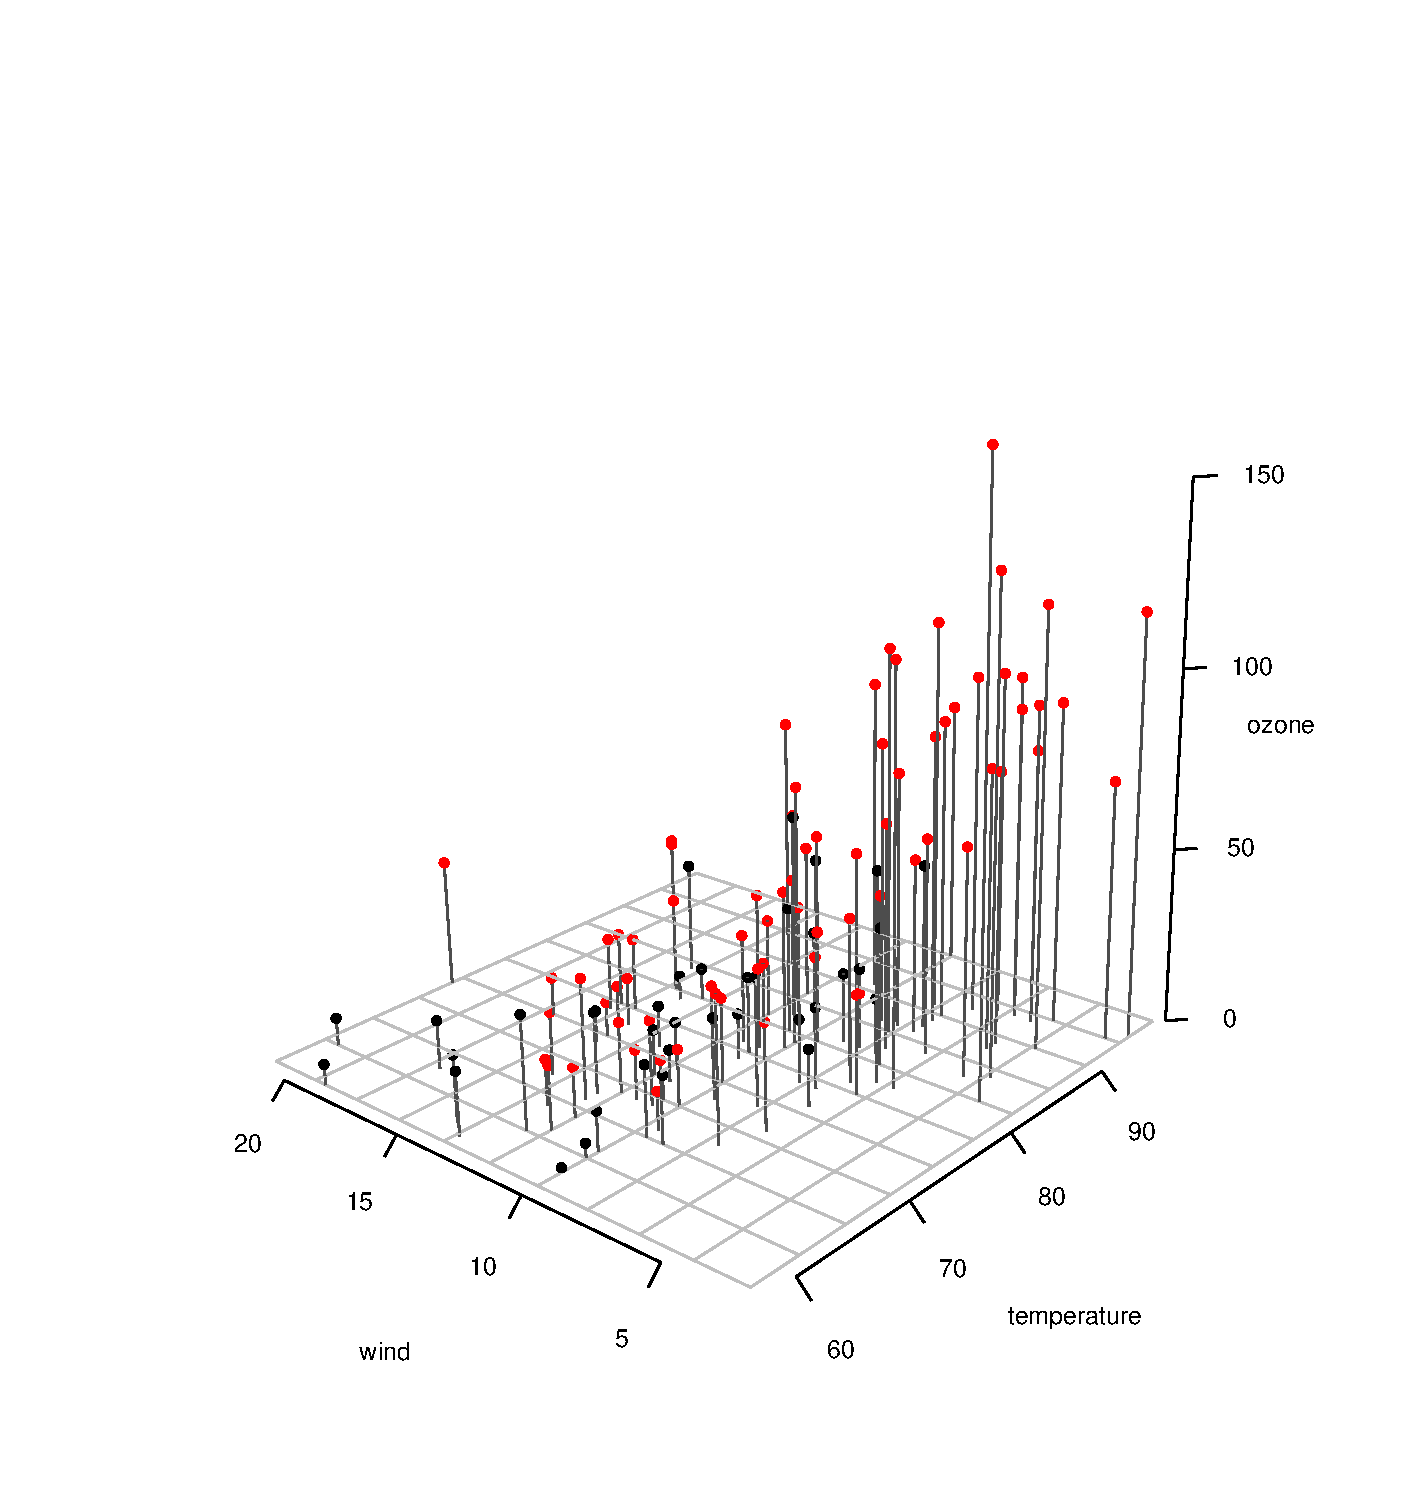
\includegraphics[scale=0.36]{figs/data.pdf}
\end{center}
\caption{Left: plot of the data. Right: plot of the first differences of the data.}
\end{figure}

\begin{figure}[H]
\begin{center}
\includegraphics[scale=0.36]{figs/spectral.pdf}
\end{center}
\caption{Left: log marginal posterior of the angular frequency $p(\omega|\m{z})$. Right: log marginal posterior of the period/wavelength $p(\lambda=2\pi/\omega|\m{z})$. The data used is the first differences (right side of Figure 1).}
\end{figure}

\subsection*{Polynomial trend model}

\noindent The DLM $\{1,1,v,vW_t\}$, with $v$ unknown, is fit to the original data $\m{y}=(y_1,\ldots,y_T)^\top$. The model is fit using the recursive formulas for normal DLMs. We integrate out $v$ at each step so that $y_t|D_{t-1}$ and $\theta_t|D_t$ follow $t$- instead of normal distributions. The recursive formulas are given in West and Harrison (1997) and Prado and West (2010).
\bigskip

\noindent We use discount factors so that $W_t=(1-\delta)/\delta C_{t-1}$, where $C_{t-1}$ is the prior scale for $\theta_{t-1}|D_{t-1}$. $\delta$ is selected by maximizing the observed predictive density
\[ p(\m{y}|D_0) = \prod_{t=1}^T p(y_t|D_{t-1}) \]
\noindent We evaluate $\log p(\m{y}|D_0)$ on the grid $\delta=\{0.500, 0.501,\ldots,1.000\}$. The plot of $\delta$ vs. $\log p(\m{y}|D_0)$ is given in Figure 3. The vertical line marks where the maximum occurs, at $\hat{\delta}=0.867$, which is chosen to be our discount factor for the remainder of the analysis.

\begin{figure}[H]
\begin{center}
\includegraphics[scale=0.34]{figs/discount.pdf}
\end{center}
\caption{The log observered predictive density evaluated across several $\delta\in[0,1]$. The dashed line indicates where the maximum occurs, at $\hat{\delta}=0.867$.}
\end{figure}

\noindent We use the priors $m_0=60$, $C_0=200$, $n_0=1$, and $d_0=100$. The values on $m_0$ and $C_0$ correspond roughly to the sample mean and variance of $\m{y}$, while the values for $n_0$ and $d_0$ are intended to be non-informative. Given $\delta=\hat{\delta}=0.867$, we summarize the filtering distribution $\theta_t|D_t$, the one-step ahead forecast distribution $y_t|D_{t-1}$, and the smoothing distribution $\theta_t|D_T$, for $t=1,\ldots,T$, in Figures 4 and 5.
\bigskip

\noindent All three distributions appear to fit the data appropriately. The filtering and the forecasts capture the general downward trend of the data as well as the semiannual wavelength. And, as expected with smoothing, we capture the trend only. The variance for the one-step ahead forecast does seem a bit too high. The bands shown in the graph are 95\% credible intervals, yet every observation falls within the bands.
\bigskip

\noindent Despite the positive appearance of these three distributions, when looking at the forecast distributions for $\theta_t$ and $y_t$ (conditioned on $D_T$), the downward trend and the seasonality is no longer present (Figure 6). The trend might be captured by using time as a covariate in $F_t$, but we run the risk of specifying a feature in the model that may not exist in the data. We could incorporate seasonality into the model by specifying $G_t$ to have a Fourier representation (P\&W p.121), using the results from the earlier spectral analysis.

\begin{figure}[H]
\begin{center}
\includegraphics[scale=0.36]{figs/current.pdf}
\end{center}
\caption{Left: mean of $\theta_t|D_t$ (thick green) with 95\% credible intervals (thin green). Right: mean of the one-step ahead forecast function $y_t|D_{t-1}$ (thick blue) with 95\% credible intervals (thin blue). Both are evaluated at $t=1,\ldots,T$.}
\end{figure}

\begin{figure}[H]
\begin{center}
\includegraphics[scale=0.36]{figs/smooth.pdf}
\end{center}
\caption{Mean of smoothing distribution $\theta_t|D_T$ (thick red) with 95\% credible intervals (thin red) at $t=T-1,\ldots,1$.}
\end{figure}

\begin{figure}[H]
\begin{center}
\includegraphics[scale=0.36]{figs/forecast.pdf}
\end{center}
\caption{Same as in Figure 4 except the darker shades indicate the forecast distributions $\theta_{T+h}|D_T$ (left) and $y_{T+h}|D_T$ (right) for $h=1,\ldots,12$.}
\end{figure}



\end{document}
